
\documentclass{article}

\usepackage[a4paper, dvips]{geometry}
\usepackage[T1]{fontenc}
\usepackage[utf8]{inputenc}
\usepackage[french]{babel}
\usepackage{amsmath,latexsym}
\usepackage{amssymb}
\usepackage{bbm}
\usepackage{hyperref}
\usepackage{enumerate}
\usepackage{xcolor}
\usepackage{pstricks}
\usepackage{pst-node}
\usepackage[amsmath, standard, hyperref, thref]{ntheorem}
%%\usepackage{french}
\usepackage{theoremref}
\usepackage{listings}
\usepackage{algorithm}
\usepackage{algpseudocode}
\usepackage{soul}
\usepackage{xcolor}
\sethlcolor{yellow}
\usepackage{csquotes}
\usepackage{graphicx}
\usepackage{float}


\graphicspath{ {./images/} }

\newcommand{\R}{\mathbbm{R}}
\newcommand{\Pv}{\mathbbm{P}}
\newcommand{\D}{\mathbbm{D}}
\newcommand{\Hv}{\mathbbm{H}}
\newcommand{\Rs}{\mathcal{R}}
\newcommand{\Fs}{\mathcal{F}}
\newcommand{\N}{\mathbbm{N}}
\newcommand{\F}{\mathbbm{F}}
\newcommand{\G}{\mathcal{G}}
\newcommand{\I}{\mathcal{I}}
\newcommand{\T}{\mathcal{T}}
\newcommand{\Ns}{\mathcal{N}}
\newcommand{\Z}{\mathbbm{Z}}
\newcommand{\Zs}{\mathcal{Z}}
\newcommand{\Q}{\mathbbm{Q}}
\newcommand{\Fpol}{\mathcal{F}_{Pol}}
\newcommand{\Flin}{\mathcal{F}/_{\equiv}}
\newcommand{\Ls}{\mathcal{L}}
\newcommand{\A}{\mathcal{A}}
\newcommand{\Ss}{\mathcal{S}}
\newcommand{\Sf}{\mathfrak{S}}
\newcommand{\B}{\mathcal{B}}
\newcommand{\E}{\mathcal{E}}
\newcommand{\K}{\mathcal{K}}
\newcommand{\C}{\mathbbm{C}}
\newcommand{\U}{\mathcal{U}}
\newcommand{\M}{\mathcal{M}}
\newcommand{\ind}{\textrm{ind}}
\newcommand{\ZFC}{\textbf{\mbox{ZFC}}}
\newcommand{\Gal}{\mathrm{Gal}}
\newcommand{\Vect}{\mathrm{Vect}}
\newcommand{\Hom}{\mathrm{Hom}}
\newcommand{\GF}{\mathrm{GF}}
\newcommand{\pgcd}{\mathrm{pgcd}}
\newcommand{\id}{\mathrm{id}}
\newcommand{\car}{\mbox{car}}
\newcommand{\gr}{\mathrm{gr}}
\newcommand{\card}{\mbox{card}}
\newcommand{\Aut}{\mbox{Aut }}
\newcommand{\Ag}{\mathfrak{A}}
\newcommand{\CD}{\textbf{\mbox{CD}}}
\newcommand{\PfN}{\mathcal{P}_f(\N)}
\newcommand{\PcofE}{\mathcal{P}_{cof}(E)}
\newcommand{\OO}{\mathcal{O}}
\newcommand{\inp}{\in_{\varphi}}
\newcounter{question}
\newcounter{subquestion}[question]
\newcounter{lemme}



\theoremstyle{break}                  % passage à la ligne 
\theorembodyfont{\itshape}     % fonte
\newtheorem{theoreme}{Théorème}
\newtheorem{preuve}{Preuve}
\newtheorem{propriete}{Propriété}
\newtheorem{lemme}{Lemme}
\newtheorem{corollaire}{Corollaire}
\newtheorem{axiome}{Axiome}
\newtheorem{rem}{Remarque}

\newtheorem{exemple}{Exemple}
\newtheorem{remarque}{Remarque}
\newtheorem{convention}{Convention}
\newtheorem{note}{Note}
\newtheorem{representation}{Représentation graphique}

\parindent=0pt

\begin{document}
\lstset{language=python}

\title{Travail d'étude et de recherche (TER)\\
M1 de Mathématiques - Sorbonne Université\\
Calcul des polynômes cyclotomiques}
\author{Jean-Philippe MERX}
\date{Mai 2025}

\maketitle

\begin{abstract}
	Ce document constitue le mémoire de mon TER effectué dans le cadre du M1 de Mathématiques de Sorbonne Université. Le TER a consisté en l'étude de l'article \cite{monagan} d'Arnold et Monagan consacré au calcul rapide des polynômes cyclotomiques. Le travail principal s'est concentré sur d'une part la compréhension des résultats mathématiques nécessaires à justifier le fonctionnement des algorithmes proposés par Arnold et Monagan et en particulier l'algorithme récursif le plus rapide, et d'autre part à analyser des éléments importants pour la mise en œuvre de cet algorithme comme la magnitude des coefficients des polynômes à calculer. Une implémentation en Python de l'algorithme a été réalisée dans le cadre du TER.
\end{abstract}

\section*{Remerciements}
Lorsque j'ai opté pour la réalisation d'un TER, j'avais à l'esprit l'étude de l'article de John Milnor sur l'existence sur la sphère de dimension 7 de structures différentielles distinctes. J'ai toujours été attiré par \emph{les bizarreries mathématiques} comme l'atteste mon site \href{https://www.mathcounterexamples.net/}{www.mathcounterexamples.net} dédié aux contre-exemples. J'ai cependant consulté avec attention la liste des TERs proposés par les enseignants du M1... et le sujet consacré au calcul des polynômes cyclotomiques a retenu mon attention. Ayant passé plusieurs années à développer des logiciels de CAO, m'arrachant les cheveux entre autres à mettre à plat des surfaces non développables et au total quarante années dans l'univers des éditeurs de logiciels, j'ai choisi cet attrayant sujet qui allie théorie et implémentation.\\

Je tiens à remercier Pierre-Vincent Koseleff d'avoir proposé ce sujet et d'avoir encadré mes activités de TER. Les échanges que nous avons eus m'ont permis d'avoir une vue plus directe du comportement des polynômes cyclotomiques, et une ouverture sur les algorithmes utilisés en calcul formel.


\section*{Introduction}
Le sujet du TER est à la jonction de l'arithmétique et du calcul formel. Pour mémoire, Pierre-Vincent Koseleff l'avait ainsi formulé:\\

\enquote{Dans [AM10], Arnold et Monagan proposent une méthode pour calculer efficacement et rapidement les polynômes cyclotomiques $\Phi_n$.
	Il s’agit de comprendre les méthodes utilisées et mises en œuvre, ainsi que d’expliquer, dans le cadre du programme du Master de Mathématiques, divers points restés obscurs ou imprécis : propriétés des polynômes cyclotomiques, irréductibilité, taille des coefficients; multiplications et divisions rapides, transformation de Fourier rapide.
	Les ouvrages [GG13, AECF, SM] pourront utilement être consultés. Le travail peut mener à des calculs explicites et un premier contact avec des logiciels de calcul formel (Sage, Maple, etc).}\\

Il s'est rapidement avéré que le sujet est vaste et que des choix étaient nécessaires. J'avais dès le départ le désir de faire intervenir une part d'implémentation dans le TER. L'un des mots clés du sujet étant \emph{calcul formel}, et me voyant difficilement calculer à la main ne serait-ce que $\Phi_{3 \cdot 5 \cdot 7 \cdot 11}$, mettre la main dans du logiciel faisait sens. Pour ce faire, la première direction qui s'est imposée à moi, a été de comprendre les algorithmes décrits dans l'article et les mathématiques sous-jacentes. Réflexe subliminal: pourquoi ça marche?  La première section de ce mémoire contient les preuves des propriétés utilisées pour les algorithmes d'Arnold et Monagan, et en particulier l'algorithme récursif \texttt{SPS4}, où SPS signifie Sparse Power Series.\\

Si pour $p < q$ premiers, les coefficients du polynôme cyclotomique $\Phi_{pq}$ appartiennent à l'ensemble $\{-1, 0, 1\}$, ce n'est pas toujours le cas pour $\Phi_n$ où $n$ est le produit de trois entiers premiers ou plus. Donc si l'on souhaite implémenter un algorithme de calcul de polynômes cyclotomiques, se pose la question de la magnitude des coefficients de ces polynômes. Et ce parce que les calculs sur des entiers de \enquote{longueur infinie} sont significativement plus lents que sur ceux de \enquote{taille machine}. En conséquence, une section du mémoire est consacrée à la hauteur des polynômes cyclotomiques. C'est un sujet vaste auquel de nombreux articles sont consacrés. Je n'en aborde dans ce mémoire qu'une petite partie. Sans avoir pu résister cependant à reproduire la preuve que tout entier est le coefficient d'un polynôme cyclotomique.\\

Une autre partie du mémoire introduit l'implémentation que j'ai réalisée en Python de l'algorithme \texttt{SPS4}. Les programmes, ainsi que l'ensemble des documents du mémoire sont accessibles dans le dépôt Git \href{https://github.com/jpmjpmjpm/cyclotom-fast}{jpmjpmjpm/cyclotom-fast}.



\section*{Mathématiques des polynômes cyclotomiques}
\subsection*{Définitions}
Pour un entier $n \ge 1$, on note $$P_n(X) = X^n - 1 \in \Q[X]$$ et $U_n$ les racines de $P_n$, c'est à dire les racines $n^{\text{ème}}$ de l'unité. $U_n$ est un sous-groupe du groupe $\mathbb U$ des complexes de module un. C'est un groupe cyclique fini. On peut le montrer en se souvenant qu'un groupe abélien fini $G$ est somme directe de ses sous-groupes $p$-maximaux $G(p)$, c'est à dire de ses éléments qui sont une puissance de $p$. Ici, on peut montrer que $G(p) = \{x \in U_n \mid x^{m_p} = 1\}$ où $m_p$ est l'ordre de $G(p)$ et donc que $G(p)$ est cyclique. On conclut sachant qu'un groupe abélien fini somme directe de groupes d'ordres premiers est cyclique.\\


On désigne dans la suite par $U_n^* \subseteq U_n$ les générateurs de $U_n$, c'est à dire les éléments dont l'ordre est exactement $n$. Le $n^{\text{ème}}$ polynôme cyclotomique $\Phi_n \in \Q[X]$ est:

$$\Phi_n(X) = \prod_{\zeta \in U^*_n} (X - \zeta) = \prod_{\substack{j=1\\ \pgcd(j,n)=1}}^n (X - e^{\frac{2 \pi i}{n}j})$$

et le $n^{\text{ème}}$ polynôme cyclotomique inverse $\Psi_n \in \Q[X]$:

$$\Psi_n(x) = \prod_{\zeta \in U_n \setminus U^*_n} (X - \zeta) = \prod_{\substack{j=1\\ \pgcd(j,n) > 1}}^n (X - e^{\frac{2 \pi i}{n}j}) = \frac{X^n - 1}{\Phi_n(X)}.$$

En particulier: $\Phi_1(X) = X-1$ et $\Psi_1(X) = 1$.\\


Dans la suite du document on note $\varphi(n)$ l'indicatrice d'Euler de $n$, qui est le degré de $\Phi_n$.

\subsection*{Propriétés utiles au calcul des polynômes cyclotomiques}
On s'attache maintenant à décrire et démontrer des propriétés des polynômes $\Phi_n, \Psi_n$ qui vont permettre de les calculer efficacement. 

\begin{propriete}\thlabel{prop:prodphi}
	Pour $n \ge 1$ on a $P_n(X) = X^n-1 = \prod_{ d \mid n} \Phi_d(X)$.
\end{propriete}
En effet, $U_n$ est la réunion des $U_d^*$ pour $d \mid n$ et les $U_d^*$ sont deux à deux disjoints.

\begin{propriete}
	Les polynômes $\Phi_n$ sont à coefficients entiers et unitaires.
\end{propriete}
Si $P, Q$ sont des polynômes à coefficients entiers, et que $Q$ est unitaire, alors il existe des polynômes $A,R$ appartenant à $\mathbb Z[X]$ tels que $P = AQ + R$. De plus, $A$ est unitaire si $P, Q$ le sont. On prouve ce résultat en appliquant l'algorithme de calcul de la division euclidienne de polynômes dans un corps et en remarquant qu'à chaque étape le terme obtenu est à coefficient entier.\\
L'utilisation de la propriété \ref{prop:prodphi} et une récurrence forte permettent de conclure que pour $n \ge 1$ $\Phi_n$ est un polynôme unitaire à coefficients entiers.

\begin{propriete}[Irréductibilité des polynômes cyclotomiques]
	Les polynômes $\Phi_n \in \mathbb Z[X]$ sont irréductibles.
\end{propriete}
On démontre cette propriété bien qu'elle ne soit pas utile pour les algorithmes utilisés ici pour leur calcul.\\

Soit $\zeta$ une racine primitive $n$-ième de l'unité, $p$ un nombre premier avec $n$ et $f,g \in \mathbb Q[X]$ les polynômes minimaux unitaires de $\zeta$ et $\zeta^p$. Montrons que $f,g$ sont à coefficients entiers. $\mathbb Z$ étant factoriel, $\mathbb Z[X]$ l'est également et $\Phi_n = f_1^{\alpha_1} \cdots f_r^{\alpha_r}$ où $f_1, \dots ,f_r \in \mathbb Z[X]$ sont supposés irréductibles. $\Phi_n$ étant unitaire, on peut supposer que les $f_i$ le sont aussi. $\zeta$ est racine de l'un des $f_i$, qui est irréductible sur $\mathbb Z$ et donc sur $\mathbb Q$. Par conséquent, $f$ est l'un des $f_i$, $g$ aussi puisque $\zeta^p$ est racine de $\Phi_n$ et $f,g$ divisent $\Phi_n$ dans $\mathbb Z[X]$.\\

Montrons que $f=g$. Dans le cas contraire, $f,g$ étant irréductibles, le produit $f \cdot g$ diviserait $\Phi_n$ dans $\mathbb Z[X]$. $\zeta^p$ étant racine de $g$, $\zeta$ est racine de $g(X^p)$ et $f(X)$ divise $g(X^p)$ dans $\mathbb Q[X]$, donc aussi dans $\mathbb Z[X]$ puisque $f$ est unitaire. On écrit $g(X^p) = f(X)h(X)$ avec $h \in \mathbb Z[X]$.\\

Projetons cette égalité dans $\mathbb F_p$. $g(X) = a_r X^r + \cdots + a_0$ avec $a_i \in \mathbb Z$. Par Frobenius:

$$\overline{g}(X^p) = (\overline{a_r} X^r + \cdots + \overline{a_0})^p = \overline{g}(X)^p = \overline{f}(X) \overline{h}(X).$$ Si $\varphi \in \mathbb F_p[X]$ est un facteur irréductible de $\overline{f}$, $\varphi$ divise $\overline{g}$ et donc $\varphi^2$ divise $\overline{\Phi}_n$ dans $\mathbb F_p[X]$. Ce qui est absurde, puisque $\overline{\Phi}_n$ divise le polynôme $X^n-1$ qui n'a que des racines simples dans un corps de décomposition lorsque $p$ ne divise pas $n$.\\

Maintenant, si $\zeta^\prime$ est une racine $n$-ième de l'unité, on a $\zeta^\prime = \zeta^m$ avec $m = p_1^{\alpha_1} \cdots p_s^{\alpha_s}$ où $p_i \nmid n$. Des applications successives de ce que l'on vient de montrer implique que $\zeta^\prime$ et $\zeta$ ont le même polynôme minimal. De sorte que $f$ admet toutes les racines primitives de l'unité comme zéro. Comme $f \mid \Phi_n$, et que ces deux polynômes sont unitaires, on obtient que $f = \Phi_n$ et que $\Phi_n$ est irréductible.\\



Notons que les polynômes cyclotomiques, ne sont pas toujours irréductibles sur les corps finis. Ainsi, sur $\mathbb F_2$:
$$\Phi_7(X)= (X^2+X^2+1)(X^3+X+1).$$\\


Nous définissons maintenant la fonction de Möbius $\mu : \mathbb N^* \to \{-1, 0, 1\}\}$:
\begin{displaymath}
	\mu(n) = :
	\begin{cases}
		1 & \text{si } n = 1\\
		0 & \text{si } n \text{ a un facteur premier carré}\\
		(-1)^r & \text{où } $r$ \text{ est le nombre de facteurs premiers de } $n$\\
	\end{cases}
\end{displaymath}

\begin{propriete}[Deux propriétés de la fonction de Möbius]
	\begin{enumerate}
		\item $\mu$ est multiplicative: si $m,n $ sont premiers entre eux: $\mu(mn)= \mu(m)\mu(n)$.
		\item Si $n >1$, $\displaystyle \sum_{d \mid n} \mu(d) = 0$.
	\end{enumerate}
\end{propriete}
Si $m$ ou $n$ est égal à $1$, la première propriété est évidente. Supposons $m,n$ premiers entre eux et plus grands que un. Si $m$ ou $n$ a un facteur premier carré,  $\mu(mn)=\mu(m)\mu(n) = 0$. Dans le cas contraire, le nombre de facteurs premiers de $mn$ est la somme des nombres de facteurs premiers de $m$ et $n$ et $\mu(mn)=\mu(m)\mu(n)$ à nouveau.\\

Concernant la seconde propriété, supposons que $n = \displaystyle \prod_{n = 1}^r p_1^{\alpha_1} \cdots p_r^{\alpha_r}$ où $\{p_1, \dots p_r\}$ sont des premiers distincts et $\alpha_1, \dots, \alpha_r$ des entiers supérieurs ou égaux à $1$. Dans la somme $\displaystyle \sum_{d \mid n} \mu(d)$, seuls les diviseurs $d$ de $n$ sans facteur premier carré ont une contribution, ce qui conduit à l'égalité:
$$\sum_{d \mid n} \mu(d) = \sum_{i = 0}^{r}\sum_{\substack{S \subseteq \{p_1, \dots, p_r\}\\ \left\vert S \right\vert = i}} (-1)^i = \sum_{i = 0}^{r} \binom{r}{i}(-1)^i =(1-1)^r=0.$$

Nous fournissons à présent une autre définition des polynômes cyclotomiques utilisant la fonction de Möbius.

\begin{propriete}[Définition équivalente des polynômes cyclotomiques]
	\begin{align}		
		\Phi_n(X) = \prod_{d \mid n} (X^d - 1)^{\mu(\frac{n}{d})} = \prod_{d \mid n} (1 - X^d)^{\mu(\frac{n}{d})} = \prod_{d \mid n} (1 - X^\frac{n}{d})^{\mu(d)} \tag{2.4}\label{mobphi}\\
		\Psi_n(X) = \prod_{d \mid n, d<n} (X^d - 1)^{-\mu(\frac{n}{d})} = -\prod_{d \mid n, d<n} (1 - X^d)^{-\mu(\frac{n}{d})}\tag{2.5}\label{mobpsi}
	\end{align}
\end{propriete}

La seconde formule est une conséquence immédiate de la première et de l'égalité $\Phi_n(X) \Psi_n(X) = X^n-1$. Pour montrer la première, notons
$$F_n(X) = \prod_{d \mid n} (X^d - 1)^{\mu(\frac{n}{d})} = \prod_{d \mid n} (X^{\frac{n}{d}} - 1)^{\mu(d)}.$$ Il suffit de prouver que $\displaystyle \prod_{ d \mid n} F_d(X) = X^n-1$, puisque l'on obtient alors par récurrence $F_n(X) = \Phi_n(X)$ partant du constat que $F_1(X) = \Phi_1(X) = 1$. Nous avons:

$$\prod_{ d \mid n} F_d(X) = \prod_{ d \mid n} \prod_{d^\prime \mid d} (X^{d^\prime} - 1)^{\mu(\frac{d}{d^\prime})}$$ et allons montrer que pour $d^\prime$ divisant $n$ fixé

$$\sum_{d \in S_d^\prime} \mu\left(\frac{d}{d^\prime}\right)=\begin{cases}1 &\text{si } d= n\\
	0 &\text{autrement }\end{cases}$$ où $S_{d^\prime} = \{d ; d^\prime \mid d \text{ et } d \mid n\}$.
Dans la somme ci-dessus, on peut changer d'indice de sommation en prenant $e = d/d^\prime$ et effectuer la somme sur l'ensemble $\overline{S}_{d^\prime} = \{e ; e \mid \frac{n}{d^\prime}\}$, c'est à dire l'ensemble des diviseurs de $\frac{n}{d^\prime}$. D'où

$$\sum_{d \in S_d^\prime} \mu\left(\frac{d}{d^\prime}\right) = \sum_{e \mid \frac{n}{d^\prime}} \mu(e)$$ et le résultat compte tenu de la seconde propriété ci-dessus de la fonction de Möbius.

Cette définition permettra le calcul des polynômes cyclotomiques en effectuant des multiplications et des divisions par des polynômes du type $X^d - 1$.

Les propriétés suivantes des polynômes cyclotomiques sont importantes pour les algorithmes de calcul. Elles permettent en effet d'une part de limiter les calculs principaux au cas où $n$ est un produit de nombres premiers distincts, et pour ce dernier cas d'élaborer un algorithme récursif pour leur calcul: l'algorithme \texttt{SPS4} de l'article étudié.


\begin{propriete}
	Soient $p,q$ des entiers premiers tels que $p \nmid n$ et $q \mid n$. Alors:
	\begin{align}
		\Phi_{np}(X) &= \frac{\Phi_n(X^p)}{\Phi_n(X)} \tag{2.8a}\label{ndivphi}\\
		\Phi_{nq}(X) &= \Phi_n(X^q) \tag{2.8b}\label{divphi}\\
		\Psi_{np}(X) &= \Psi_n(X^p)\Phi_n(X) \tag{2.8c}\label{ndivpsi}\\
		\Psi_{nq}(X) &= \Psi_n(X^q)	 \tag{2.8d}\label{divpsi}
	\end{align}
\end{propriete}

Remarquons tout d'abord que si $m$ est un entier quelconque
$$\Phi_{nm}(X) \Psi_{nm}(X) = X^{nm}-1 = (X^p)^m-1=\Phi_{n}(X^m) \Psi_{n}(X^m).$$ Si $\ref{ndivphi}$ est vraie on obtient
$$\Psi_{np}(X) = \frac{X^{np}-1}{\Phi_{np}(X)} =\frac{X^{np}-1}{\Phi_{n}(X^p)}\Phi_n(X)=\Psi_n(X^p)\Phi_n(X)$$ montrant $\ref{ndivpsi}$. De manière similaire, on déduit $\ref{divpsi}$ de $\ref{divphi}$.\\

Pour $n$ entier, nous noterons dorénavant $D_n$ l'ensemble des diviseurs de $n$ sans facteurs carré. On peut réécrire \ref{mobphi}
$$\Phi_{n}(X) = \prod_{d \in D_n} (1 - X^\frac{n}{d})^{\mu(d)}.$$ Si $d$ est un diviseur sans facteur carré de $np$, ou bien $d$ divise $n$, ou bien $d$ est de la forme $d^\prime p$. D'où l'égalité
$$\Phi_{np}(X) = \prod_{d \in D_{n}} (1 - X^\frac{np}{d})^{\mu(d)}
\prod_{dp \in D_{np}} (1 - X^\frac{np}{dp})^{\mu(dp)}.$$ Le premier facteur est $\Phi_{n}(X^p)$. Observons que dans le second, $dp$ étant sans facteurs carré, $d$ est premier avec $p$ et donc $\mu(dp)= \mu(d)\mu(p)= - \mu(d)$. Ce second facteur est simplement l'inverse de $\Phi_{n}$: nous avons prouvé $\ref{ndivphi}$.\\

Il nous reste à prouver $\ref{divphi}$. Puisque $q$ divise $n$, les diviseurs sans facteurs carré de $nq$ sont ceux de $n$ et
$$\Phi_{nq}(X) = \prod_{d \in D_{n}} (1 - X^\frac{nq}{d})^{\mu(d)} = \Phi_n(X^q),$$ qui est le résultat souhaité.\\

\textbf{Remarque:} il est aussi possible de démontrer ces formules sans faire appel aux formules closes en raisonnant sur les propriétés des racines primitives de l'unité.\\

Portant notre attention sur le cas où $2$ divise $n$, nous allons obtenir la propriété suivante:


\begin{propriete}\thlabel{prop:oddprime}
	Pour $n > 1$:
	$$\Phi_{2n}(X) = \begin{cases}
		\Phi_n(X^2) & \text{si } $n$ \text{ est pair}\\
		\Phi_n(-X) & \text{sinon}
	\end{cases}$$
\end{propriete}

Le cas $n$ pair est une application immédiate de $\ref{divphi}$. Si $n$ est impair, les polynômes $\Phi_{2n}(X)$ et $\Phi_{n}(-X)$ sont égaux puisqu'ayant les mêmes racines qui sont simples. Ce résultat nous permet de nous concentrer sur le calcul des polynômes cyclotomiques $\Phi_n$ avec $n$ impair.\\

On déduit d'autre part des formules précédentes $\ref{divphi}$ et $\ref{divpsi}$ pour le cas où $q \mid n$ que


\begin{propriete}[Réduction aux cas des entiers sans facteurs carré]\thlabel{prop:nosquare}
	Si $n = q_1^{e_1} \cdots q_k^{e_k}$ où $q_1, \dots, q_k$ sont des premiers distincts:
	\begin{align*}
		\Phi_{n}(X) &= \Phi_{q_1 \cdots q_k}(X^{q_1^{e_1 - 1} \cdots q_k^{e_k - 1}})\\
		\Psi_{n}(X) &= \Psi_{q_1 \cdots q_k}(X^{q_1^{e_1 - 1} \cdots q_k^{e_k - 1}})
	\end{align*}
\end{propriete}

Cette propriété et la précédente permettent de limiter le calcul des polynômes cyclotomiques au cas où $n$ est un produit de nombres premiers impairs distincts.\\


Pour ce faire, supposons que $n = p_1 \cdots p_k$ soit le produit de $k$ nombres premiers \textbf{impairs} distincts. Pour $1 \le i \le k$, notons $m_i = p_1 \cdots p_{i-1}$ et $e_i = p_{i+1} \cdots p_{k}$. En particulier $m_1=e_k=1$ et on note $e_0 = n$. Pour $1 \le i \le k$, nous avons alors $n = e_i p_i n_i$, ainsi que $e_{i-1}=p_i e_i$ et $m_{i+1}=m_i p_i$. À partir de la formule $\ref{ndivphi}$ et de l'identité $\Phi_{m_k}(X) \Psi_{m_k}(X) = X^{m_k}-1$ on obtient
$$\Phi_{n}(X) = - \frac{\Psi_{m_k}(X^{e_k})}{1- X^{n/p_k}} \Phi_{m_k}(X^{e_{k-1}}).$$
Sachant que $\Phi_1(X^{e_0}) = \Phi_1(X^n) = X^n-1$ on montre alors par récurrence:
$$\Phi_n(X)=\prod_{j=1}^{k} - \Psi_{m_j}(X^{e_j}) \prod_{j=1}^{k} (1-X^{n/p_j})^{-1}(1-X^n)$$
ou encore $$\Phi_n(X)=\prod_{j=2}^{k} - \Psi_{m_j}(X^{e_j}) \prod_{j=1}^{k} (1-X^{n/p_j})^{-1}(1-X^n)$$
puisque $\Psi_{m_1}(X^{e_1}) = \Psi_{1}(X^{e_1}) =1$. L'utilisation de la formule $\ref{ndivpsi}$ et une récurrence similaire permet d'écrire $\Psi_n(X)$ comme produit de polynômes cyclotomiques d'ordres inférieurs; ce que l'on résume dans la propriété suivante:


\begin{propriete}[Formules récursives de calcul des polynômes cyclotomiques]
	\begin{align*}
		\Phi_n(X) &=\prod_{j=2}^{k} - \Psi_{m_j}(X^{e_j}) \prod_{j=1}^{k} (1-X^{n/p_j})^{-1}(1-X^n)\tag{3.17}\label{recurphi}\\
		\Psi_{n}(X) &=\prod_{j=1}^{k} \Phi_{m_j}(X^{e_j})\tag{3.25}\label{recurpsi}
	\end{align*}
\end{propriete}

\begin{propriete}[Palindromie des polynômes cyclotomiques]
	Pour $n > 1$ impair, le polynôme $\Phi_n(X) = \sum_{i=0}^{\varphi(n)} a_i X^i$ est palindromique tandis que $\Psi_n(X) = \sum_{j=0}^{n-\varphi(n)} b_j X^j$ est anti-palindromique, ce qui signifie que
	$$a_i=a_{\varphi(n)-i} \text{ et } b_j=-b_{n-\varphi(n)-j}.$$
\end{propriete}
Si $\omega$ est une racine primitive $n$-ième de l'unité, $\omega^{-1}$ aussi. $n$ étant supposé impair, $\omega \neq \omega^{-1}$ et le produit des racines de $\Phi_{n}$ est égal à $1 = a_0$ puisque $\varphi(n)$ est pair pour $n > 2$. $X^{\varphi(n)} \Phi_n(\frac{1}{X})$ est un polynôme unitaire, dont les racines sont exactement celles de $\Phi_n(X)$, ce qui prouve que $\Phi_n(X)$ est palindromique.\\

De l'égalité $\Phi_n(X)\Psi_n(X) = X^n-1$ il résulte d'une part que $\Psi_n(X)$ est unitaire et d'autre part que $b_0=-1$. On remarque aussi que si $\zeta$ n'est pas une racine primitive $n$-ième de l'unité, alors $\zeta^{-1}$ non plus. $-X^{n-\varphi(n)} \Psi_n(\frac{1}{X})$ est donc un polynôme unitaire, comme $\Psi_{n}(X)$ et qui possède précisément les racines de $\Psi_{n}(X)$. Ces deux polynômes sont donc égaux, et nous concluons que $\Psi_{n}(X)$ est anti-palindromique.


\begin{propriete}[Produit de polynômes palindromiques / anti-palindromiques]
	Le produit de deux polynômes palindromiques ou anti-palindromiques est palindromique.\\
	Le produit d'un polynôme palindromique par un polynôme anti-palindromique est anti-palindromique.
\end{propriete}
Démonstration claire à partir des définitions. 

\section*{Calcul des polynômes cyclotomiques}
Comme mentionné à la section précédente, les propriétés \ref{prop:oddprime} et \ref{prop:nosquare} permettent de restreindre les calculs aux polynômes cyclotomiques $\Phi_n$ pour $n$ impair et sans facteur carré. C'est l'hypothèse constamment retenue par Arnold et Monagan dans les algorithmes qu'ils présentent. On décrit maintenant succinctement les algorithmes de l'article pour se concentrer ensuite sur le dernier à savoir \texttt{SPS4}.\\

Le premier, utilise de manière itérative la formule $\ref{ndivphi}$, à savoir:
$$\Phi_{np}(X) = \frac{\Phi_n(X^p)}{\Phi_n(X)}$$ où $p$ premier ne divise pas $n$. La mise en œuvre de cet algorithme nécessite des divisions de polynômes. C'est la méthode utilisée pour calculer les polynômes cyclotomiques du package Python \href{https://docs.sympy.org/latest/index.html}{SymPy}. Dans ce package, la division des polynômes est effectuée par \enquote{division euclidienne classique}. Arnold et Monagan mentionnent que de leur côté, il ont implémenté cet algorithme en faisant appel à la FFT et à la méthode de Newton appliquée aux séries formelles pour les divisions de polynômes selon \cite{algocomputalg}.\\

Les autres algorithmes de l'article s'appuient sur la formule close $\ref{mobphi}$:
$$\Phi_n(X) =  \prod_{d \mid n} (1 - X^d)^{\mu(\frac{n}{d})}.$$
L'algorithme \texttt{SPS} utilise directement cette formule et la palindromicité de $\Phi_n$. Cependant, les calculs sont effectués à chaque étape sur l'ensemble des coefficients de $\Phi_n$, qui rappelons le sont au nombre de $\varphi(n)+1$. L'algorithme \texttt{SPS-Psi} est le pendant de \texttt{SPS} pour les polynômes cyclotomiques inverses.\\

L'algorithme \texttt{SPS2} utilise la formule:
$$\Phi_{mp}(X) = - \Psi_m(X) \Phi_m(X^p) \frac{1}{1 - X^m}.$$ Si bien que pour calculer $\Phi_{n}$ où $n = mp$ et $p$ le plus grand diviseur premier de $n$, on peut utiliser la procédure \texttt{SPS-Psi} sur un polynôme de degré $m - \varphi(m)$ au lieu d'effectuer des calculs sur des polynômes de degré $\varphi(n)$. Cependant, cet avantage n'est utilisé qu'une fois pour $\Psi_m(X)$.\\

L'algorithme \texttt{SPS3} utilise quant à lui ce bénéfice de manière itérative en appliquant la formule précédente à $\Phi_m(X^p)$.\\

L'article d'Arnold et Monagan compare les performances des algorithmes proposés en fournissant un tableau contenant les temps de calcul pour différents polynômes cyclotomiques. Cependant, il n'y a pas d'analyse détaillée des échelles en temps des algorithmes. Ces échelles de temps sont mentionnées dans une autre version de l'article \cite{monagan+}.\\

Dans la suite de cette section, on décrit la méthode utilisée dans l'algorithme \texttt{SPS4} de l'article pour calculer de manière rapide les polynômes cyclotomiques, ainsi qu'une implémentation effectuée en Python. On commence par quelques considérations techniques.

\subsection*{Éléments techniques à prendre en compte}

Le calcul d'un polynôme cyclotomique d'ordre $n$ comportant des facteurs carrés s'effectue en utilisant la propriété \ref{prop:nosquare}. Dans ce cas, on obtient des polynômes creux. Par souci d'économie de mémoire, on utilise alors une représentation sous la forme par exemple de dictionnaires plutôt que de simples tableaux. C'est ce qui est réalisé dans l'implémentation  
SAGE \href{https://github.com/sagemath/sage/blob/develop/src/sage/rings/polynomial/cyclotomic.pyx}{\texttt{cyclotomic.pyx}}.\\

On cherche donc à calculer de manière rapide les polynômes cyclotomiques $\Phi_n$ pour lesquels $n$ "est grand". Mais qu'entend-on par grand? Il y a au moins deux éléments importants à considérer.\\

Tout d'abord l'espace mémoire nécessaire pour le stockage d'un polynôme cyclotomique $\Phi_n$. Si $n = p_1 \cdots p_k$ où $p_1, \dots, p_k$ sont $k$ premiers impairs distincts, le degré de $\Phi_n$ est égal à l'indicatrice d'Euler $\varphi(n) = (p_1-1) \cdots (p_k-1)$. Ainsi pour $n = 3 \cdot 5 \cdot 7 \cdot 11 \cdot 13 \cdot 17 \cdot 19 \cdot 23 \cdot 29$, le degré de $\Phi_n$ est égal à $1,021,870,080$ et à supposer que chacun des coefficients de $\Phi_n$ tienne sur 64 bits, on obtient un polynôme nécessitant 8 Go de mémoire. On approche ici des limites de ce qui calculable en mémoire vive sur un ordinateur personnel.\\

Un autre paramètre majeur pour les implémentations est la magnitude des coefficients de $\Phi_n$. On désigne par $A(n)$ la hauteur de $\Phi_n$, c'est à dire la valeur maximale des valeurs absolues des coefficients de $\Phi_n$. Nous verrons que l'algorithme \texttt{SPS4} n'utilise que des calculs sur les entiers et que seules des additions (et soustractions) sont mises en œuvre. Encore faut-il pour obtenir des calculs rapides que les entiers sur lesquels on travaille puissent-être représentés par des "entiers machine", ce qui veut généralement dire en 2025 sur 64 bits. Si ce n'est pas le cas, on fait face à un dilemme. Ou bien l'on travaille en précision entière infinie (ce qui est le cas par défaut de Python), mais on perd beaucoup en rapidité. Ou bien on teste dans tous les calculs l'overflow, ce qui est mieux, mais cependant plus lent que d'effectuer directement les additions et soustractions. L'écart de rapidité est cependant ici simplement proportionnel. Une troisième méthode est possible. Elle consiste à avoir calculé par un programme où l'on se prémunit de l'overflow le plus petit $n$, nommé $n_{64}$ pour lequel $A(n)$ reste représentable sur 64 bits, puis dans le \textit{programme définitif}, à mettre en place un calcul différent selon que l'on souhaite calculer $\Phi_n$ avec $n \ge n_{64}$ ou $n < n_{64}$.\\


C'est cette troisième stratégie qui est implémentée dans SAGE. \texttt{cyclotomic.pyx} utilise les résultats suivants de Michael Monagan:
\begin{itemize}
	\item Pour $n<10163195$, $A(n)$ est inférieure ou égale à 74989473, soit 26.16 bits, et on peut effectuer les calculs en 32 bits.
	\item Pour $n=10163195$, $A(n)=1376877780831$,  soit 40.32 bits.
	\item Si $n < 169,828,113$, $A(n)$ tient sur 60 bits.
	\item Pour $n = 169828113$, on obtient une hauteur égale à $31484567640915734951$ qui nécessite 65 bits pour être représenté. Dans ce dernier cas, \texttt{cyclotomic.pyx} bascule sur l'utilisation de PARI avec le joli warning: \texttt{print("Warning: using PARI (slow!)")}.\\
\end{itemize}

On le voit, la hauteur $A(n)$ est importante pour la mise en œuvre d'un algorithme de calcul rapide des polynômes cyclotomiques. Pour $n \ge 3 \cdot 7 \cdot 13 \cdot 17 \cdot 23 \cdot 37 \cdot 43 = 169828113$, on n'est plus à même d'utiliser l'arithmétique 64 bits des machines. Il est alors nécessaire d'invoquer des méthodes de calcul en arithmétique infinie.\\

On aborde dans une section dédiée la question de la hauteur des polynômes cyclotomiques. Revenons pour le moment à l'algorithme \texttt{SPS4}.

\subsection*{Algorithme \texttt{SPS4}}
L'algorithme \texttt{SPS4} de l'article est récursif basé sur la formule \ref{recurphi} qui permet de calculer un polynôme cyclotomique à partir de polynômes cyclotomiques inverses d'ordres inférieurs et de la formule \ref{recurpsi} qui donne un polynôme cyclotomique inverse comme produit de polynômes cyclotomiques d'ordres inférieurs. L'algorithme alterne l'utilisation des polynômes cyclotomiques et cyclotomiques inverses.\\

Prenons par exemple $n = 3 \cdot 5 \cdot 7 = 105$. On obtient successivement les équations:
\begin{align*}
	\Phi_{105}(X) &= \Psi_{15}(X)\Psi_{3}(X^7)(1-X^{105})(1-X^{15})^{-1}(1-X^{21})^{-1}(1-X^{35})^{-1}\\
	\Psi_{15}(X) &= \Phi_{5}(X) \Phi_{1}(X^3)\\
	\Psi_{3}(X^7) &= \Phi_{1}(X^7) 
\end{align*}

En analysant le processus récursif, on constate qu'une seule procédure récursive est suffisante pour effectuer ces calculs si elle possède un paramètre permettant de choisir une récursion sur un polynôme cyclotomique ou sur un polynôme cyclotomique inverse.\\

\textbf{Au terme de ce processus récursif, les seules opérations arithmétiques utilisées sont des additions et des soustractions.} En effet, dans les formules \ref{recurphi} et \ref{recurpsi}, on n'effectue effectivement que des multiplications par des polynômes de la forme $(1-X^d)$ et des divisions par de tels polynômes. Mais diviser par $(1-X^d)$, revient à multiplier par la série formelle $\displaystyle \sum_{k = 0}^\infty X^{kd}$ en s'arrêtant à un nombre de termes suffisants. C'est à dire $\varphi(n)$ pour le calcul de $\Phi_n(X)$ ou $n - \varphi(n)$ pour celui de $\Psi_n(X)$.\\


\par La procédure récursive est la suivante:

\begin{figure}[H]
	\centering
	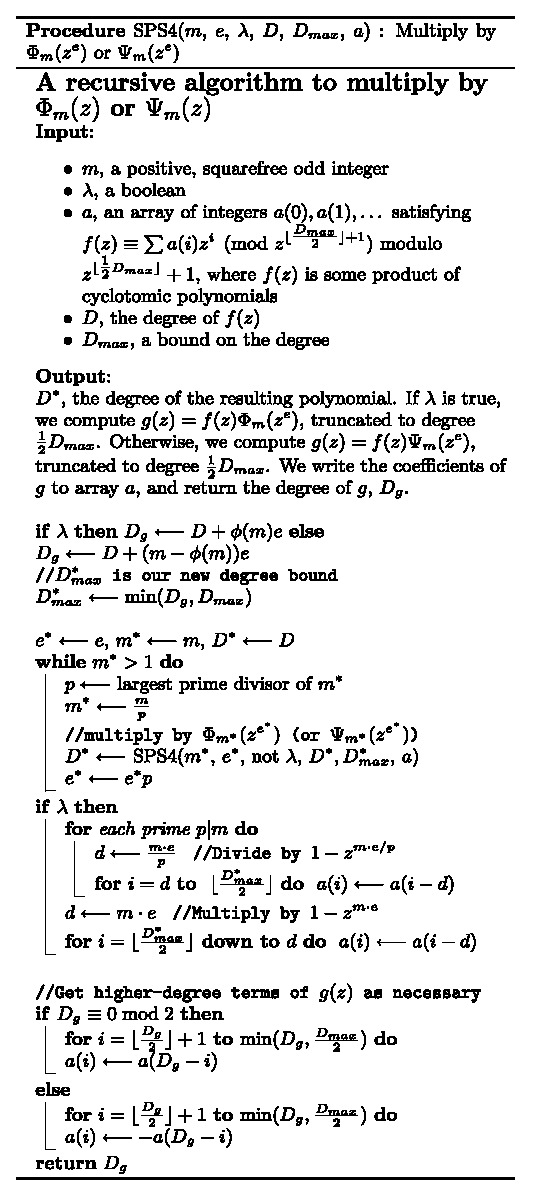
\includegraphics{cyclotomic-highperf-sps4.eps}
\end{figure}

Dans cet algorithme, la division par $1- X^d$ est effectuée en une seule boucle, ce qui m'avait intrigué. La raison en est la suivante. Supposons que $B(X) = \sum_{i=0}^\infty b_i X^i$ soit une série formelle (ou un polynôme) et que l'on cherche à calculer $C(X) = B(X) (1-X^d)^{-1}$. On a:
\begin{align*}
	C(X) &= \sum_{i=0}^\infty c_i X^i=B(X) (1-X^d)^{-1}\\
	&= \left(\sum_{i=0}^\infty b_i X^i\right)\left(1 + X^d + X^{2d} + \cdots\right)\\
	&= \sum_{i=0}^\infty\left(b_i + b_{i-d} + b_{i-2d} + \cdots\right) X^i
\end{align*}

On observe que le terme de degré $i$ de $C(X)$ ne dépend que des termes de degré inférieur ou égal de $B(X)$. En particulier, $c_i = b_i$ pour $0 \le i \le d$. Pour $i > d$ et $q = \sup \{r \ge 0 \mid i-rd \ge 0\}$:
$$c_i = b_i + b_{i-d} + \cdots + b_{i-qd}$$ tandis que
$$c_{i-d} = b_{i-d} + b_{i-d} + \cdots + b_{i-qd}.$$ D'où
$$c_i = c_{i-d} + b_i$$ pour $i > d$. On obtient un calcul en temps linéaire au lieu d'un temps quadratique par la méthode naïve qui recalcule de manière inutile des termes intermédiaires.\\

J'ai réalisé une implémentation en Python disponible dans le dépôt Git \href{https://github.com/jpmjpmjpm/cyclotom-fast/blob/master/cyclotomfast/sps4.py}{sps4.py}. J'ai validé son fonctionnement en vérifiant que la hauteur des polynômes calculés est bien celle fournie dans l'article d'Arnold et Monagan. Cette version n'est qu'un prototype qui pourrait-être amélioré d'une part en n'allouant qu'une fois la mémoire nécessaire au calcul du polynôme cyclotomique et d'autre part en faisant appel à la compilation pour les boucles internes de calcul.\\

\section*{Hauteur des polynômes cyclotomiques}\label{sec:hauteur}
Dans cette section, on étudie la magnitude des coefficients des polynômes cyclotomiques $\Phi_n(X)$. Dans un premier temps, pour $n$ premier ou produit de deux entiers premiers. Dans un second temps, on énoncera des résultats concernant la croissance asymptotique de la hauteur $A(n)$ des polynômes cyclotomiques.\\


On constate que pour $p$ premier:
$$\Phi_p(X) = \frac{X^p-1}{\Phi_1(X)} = \frac{X^p-1}{X-1} = \sum_{k=0}^{p-1} X^k,$$
et tous les coefficients de $\Phi_p(X)$ sont égaux à $1$. Si $n$ est produit de deux entiers premiers $p,q$, on va montrer que les coefficients du polynôme cyclotomique:
$$\Phi_{pq}(X) = \frac{(1-X)(1-X^{pq})}{(1-X^p)(1-X^q)}$$ sont dans $\{-1, 0, 1\}$. Le degré de $\Phi_{pq}(X)$ est égal à $(p-1)(q-1)$. En considérant l'égalité précédente dans l'anneau $\mathbb Z[[X]]$, où la division par $(1-X^p)(1-X^q)$ a un sens puisque le coefficient constant est égal à un, les coefficients de $\Phi_{pq}(X)$ sont donc ceux de $(1-X)(1-X^p)^{-1}(1-X^q)^{-1}$ tronqués à l'ordre $\varphi(pq)$. Prouvons tout d'abord que les coefficients $a_m$ de la série formelle
$$S_{pq}(X) = (1-X^p)^{-1}(1-X^q)^{-1} = \sum_{m \ge 0} a_m X^m$$ sont égaux à zéro ou un pour $0 \le m < pq$. Il suffit pour cela de montrer qu'il existe au plus un couple d'entiers $(a,b) \in \mathbb N^2$ tel que $ap+bq = m$ pour $0 \le m < pq$. Or le lemme de Gauss implique que si $ap+bq = a^\prime p + b^\prime q$, il existe $r$ entier tel que $a^\prime = a -rq$ et $b^\prime = b +rp$. Sans perte de généralité, on peut supposer $b^\prime \ge b$, c'est à dire $r \ge 0$. L'hypothèse $m <pq$ implique
$$pq > a^\prime p + b^\prime q \ge (b + r p)q \ge rpq$$ d'où $r=0$ et $(a,b)=(a^\prime, b^\prime)$.

Les coefficients de $\Phi_{pq}(X)$ sont ceux de $(1-X) S_{pq}(X)$ tronqués à l'ordre $\varphi(pq)$. Étant différence de deux entiers de $\{0,1\}$, ils appartiennent à $\{-1,0,1\}$, ce que nous souhaitions prouver. Cette démonstration s'appuie sur un sujet de préparation à l'agrégation \cite{agreg}.  Notons que la réciproque est fausse: $\Phi_{651} = \Phi_{3 \cdot 5 \cdot 31}$ est un polynôme cyclotomique d'ordre le produit de trois premiers distincts dont les coefficients sont dans $\{-1,0,1\}$.\\

On dit de $\Phi_{pq}$ dont l'ordre est produit de deux premiers distincts qu'il est binaire. Et de $\Phi_{pqr}$ qu'il est ternaire. $\Phi_{105} = \Phi_{3 \cdot 5 \cdot 7}$ est en quelque sorte le premier polynôme cyclotomique ternaire d'ordre impair. $-2$ est l'un de ses coefficients. N'importe quel entier est-il le coefficient d'un polynôme cyclotomique? La réponse est positive et on reproduit ici la preuve de cet article de Jiro Suzuki \cite{range}.\\

On note $C$ les valeurs prises par l'ensemble des coefficients de tous les polynômes cyclotomiques et on commence par prouver que
\begin{propriete}
	pour tout entier $t > 2$, il existe $t$ nombres premiers distincts $p_1 < p_2 < \cdots < p_t$ tels que $p_1+p_2 > p_t$.
\end{propriete}
Dans le cas contraire, il existerait un entier $t > 2$ tel que pour tous premiers vérifiant $p_1 < p_2 < \cdots < p_t$ on ait $p_1+p_2 \le p_t$ et donc $2 p_1 < p_t$. Cela implique que pour tout entier $k$, il y a au plus $t$ nombres premiers entre $2^{k-1}$ et $2^k$ et que $\pi(2^k) < kt$, contrairement à ce qu'affirme le théorème des nombres premiers à savoir: 
$$\pi(n) \underset{n \to \infty}{\sim} \frac{n}{\ln n}.$$

Revenons à notre affirmation initiale qui spécifie que tout entier $s \in \mathbb Z$ est le coefficient $c_i^{(n)}$ d'un polynôme cyclotomique $\Phi_n$. Soit $t$ un entier impair supérieur à 2 et $t$ nombres premiers $p_1 < p_2 < \cdots < p_t$ tels que $p_1+p_2 > p_t$. Notons $p = p_t$ et $n = p_1 p_2 \cdots p_t$. On a
$$\Phi_n(X) = \prod_{d \mid n} (1-X^d)^{\mu(\frac{n}{d})} = \sum_{i = 0}^{\varphi(n)} c_i^{(n)} X^i.$$
Pour $r > s$, on a $p_r + p_s > p_t = p$ et par conséquent
\begin{align*}
	\Phi_n(X) &\equiv \prod_{i=1}^{t} (1-X^{p_i})/(1-X) &(\mathrm{mod} \, X^{p+1})\\
	&\equiv (1 + X + \cdots + X^p)(1 - X^{p_1}-X^{p_2}-\cdots-X^{p_t})  &(\mathrm{mod} \, X^{p+1}).
\end{align*}
On constate que $c_p^{(n)}=-t+1$ et $c_{p-2}^{(n)}=-t+2$ ce qui montre que $\{s \in \mathbb Z \mid s \le -1\} \subseteq C$ puisque $t$ est n'importe quel nombre naturel impair supérieur ou égal à $3$.\\

On sait d'autre part que pour $m$ entier positif impair
$$\Phi_{2m}(X) = \Phi_m(-X).$$
Si $p_1 \ge 3$, $n = p_1 p_2 \cdots p_t$ est impair, $c_p^{(2n)}=t-1$ et $c_{p-2}^{(2n)}=t-2$. On en déduit que $\{s \in \mathbb Z \mid s \ge 1\} \subseteq C$. Et finalement que $C = \mathbb Z$ puisque $c_2^{15} = 0$.\\

Dans la preuve ci-dessus, on augmente indéfiniment le nombre de facteurs premiers $t$ de $n$ pour exhiber un coefficient arbitrairement grand d'un polynôme cyclotomique $\Phi_n$. Emma Lehmer démontra en 1936 \cite{infini} que les coefficients des polynômes cyclotomiques ternaires forment un ensemble infini. Pour montrer que $\limsup\limits_{n \to \infty} A(n) = \infty$, il "suffit" de considérer les polynômes cyclotomiques ternaires.\\

Le mathématicien suédois Carl Severin Wigert a prouvé que:
$$\limsup\limits_{n \to \infty} \frac{\log d(n)}{\log n / \log \log n} = \log 2$$ où $d(n)$ désigne le nombre de diviseurs de $n$; voir par exemple le théorème 317 de  \cite{numbers}. On utilise ce résultat pour établir (en suivant le mathématicien américain Paul T. Bateman) que

\begin{propriete}
	$$\limsup\limits_{n \to \infty} A(n) \le \exp(n^{\log 2 / \log \log n}).$$
\end{propriete}

Partons de nouveau de l'égalité $\Phi_n(X) = \prod_{d \mid n} (1-X^d)^{\mu(\frac{n}{d})}$ et remarquons que
\begin{itemize}
	\item la hauteur d'un polynôme $P$ produit de polynômes $P_i = \sum_{j=0}^{n_i} p_j^{(i)} X^j$ est inférieure ou égale à la hauteur du polynôme $Q$ produit des polynômes $\widetilde{P_i} = \sum_{j=0}^{n_i} \lvert p_j^{(i)} \rvert X^j$,
	\item $1/(1-X^d)$ est égale à la série formelle $\sum_{k \ge 0} X^{kd}$, et les termes de degré supérieurs à $\varphi(n)$, donc supérieurs ou égaux à $n$ ne contribuent pas au calcul de $\Phi_n$.\\
\end{itemize}
On déduit de cela que la hauteur de $\Phi_n$ est inférieure ou égal à celle du polynôme
$$\Delta_n(X) = \prod_{d \mid n} (1 + X^d + X^{2d} + \cdots + X^{(n/d - 1)d}).$$
La hauteur d'un produit de polynômes dont les coefficients sont tous égaux à un étant moindre que le produit des valeurs de ces polynômes en un (ce que l'on prouve par récurrence sur le nombre de polynômes), on obtient en utilisant le résultat de Carl Severin Wigert mentionné plus haut:

\begin{align*}
	A(n) &< \prod_{d \mid n} (n/d) = n^{d(n)/2} = \exp\left(\frac{1}{2}d(n) \log n\right)\\
	&< \exp\left(\frac{1}{2}2^{(1+\epsilon/2)\log n/ \log \log n}\log n\right)\\
	&< \exp\left(2^{(1+\epsilon)\log n/ \log \log n}\right)\\
	&= \exp\left(n^{(1+\epsilon)\log 2/ \log \log n}\right)
\end{align*}

pour tout $\epsilon > 0$ et $n$ suffisamment grand, ce qui permet de conclure.\\

Le mathématicien britannique Robert Charles Vaughan a lui prouvé que pour une infinité d'entiers $n$
$$A(n) > \exp\left(n^{\log 2/ \log \log n}\right).$$

\section*{Conclusion}
L'article d'Arnold et Monagan m'a intéressé à de nombreux titres. Il permet de découvrir de multiples facettes des polynômes cyclotomiques au travers d'algorithmes pour leur calcul. À ce sujet, la \enquote{survey} \cite{survey} de Carlo Sanna est une mine d'or.\\

Après avoir passé quelques semaines au côté de cet article, j'ai l'impression d'y découvrir en filigrane le cheminement de la pensée des deux auteurs. Lorsque en 2010 Arnold et Monagan ont entamé leurs travaux, il fallait cinq minutes à Maple 13 pour calculer $\Phi_{255255}(X)$... et une seconde après qu'ils aient mis en œuvre leur algorithme.\\

On comprend que la méthode qui vient rapidement à l'esprit pour calculer $\Phi_n$ est basée sur la formule:
$$\Phi_{np}(X) = \frac{\Phi_n(X^p)}{\Phi_n(X)}$$ et qu'alors la rapidité des divisions de polynômes est un facteur critique. Arnold et Monagan exploitent de manière intense cette première voie. Puis ils explorent une autre route utilisant la formule close qui caractérise les polynômes cyclotomiques. Ce qui présente de nombreux avantages. En particulier de n'utiliser que des additions et des soustractions dans les calculs. Cependant, la formule close masque partiellement les bénéfices d'un calcul itératif. Ils cherchent alors à les retrouver en mixant les deux options.\\

Maintenant, ils sont à même de calculer en un temps court des polynômes cyclotomiques qui ne sont plus que de simples jouets! Surgi le problème de la magnitude des coefficients des polynômes cyclotomiques et les difficultés matérielles. Un ordinateur travaille vite sur des entiers 64 bits. Estimer la hauteur des polynômes cyclotomiques devient essentiel.\\

J'ai aussi apprécié de mettre en œuvre l'algorithme \texttt{SPS4}. Cela m'a permis de comprendre de manière concrète son fonctionnement. Il est satisfaisant de voir s'afficher en une seconde les 92161 coefficients de $\Phi_{255255}(X)$!\\

Et ensuite? J'achève un nouveau M1 cette année, dans une position d'étudiant un peu atypique, à soixante ans passés. Avec toujours cet intérêt pour les mathématiques qui ne m'a jamais quitté ainsi que ce goût de l'ingénieur pour produire des choses concrètes fût-ce du logiciel.\\

Alors pourquoi ne pas participer à des travaux en calcul formel en tant que retraité; histoire de ne pas aller à la pêche tous les jours. L'avenir le dira.


\begin{thebibliography}{9}
	\bibitem{monagan+}
	Andrew Arnold et Michael Monagan (2011)
	\emph{Calculating cyclotomic polynomials}, Mathematics of computation - Volume 80, Number 276.
	
	\bibitem{monagan}
	Andrew Arnold et Michael Monagan (2010) \href{https://wayback.cecm.sfu.ca/~ada26/cyclotomic/PDFs/highperf.pdf}{\emph{A high-performance algorithm\\ for calculating cyclotomic polynomials}}, Simon Fraser University -	Burnaby, B.C. Canada.
	
	\bibitem{agreg}
	Pierre Charollois (2015) \href{https://webusers.imj-prg.fr/~pierre.charollois/Charollois_Pbme_cyclotomiques_agreg2015.pdf}{\emph{Problème de Mathématiques Générales no. 2.}}, Université Pierre et Marie Curie.
	
	\bibitem{survey}
	Carlo Sanna (2021) \href{https://arxiv.org/pdf/2111.04034}{\emph{A Survey on Coefficients of Cyclotomic Polynomials}}, Politecnico di Torino.
	
	\bibitem{range}
	Jiro Suzuki (1987) \href{https://projecteuclid.org/journals/proceedings-of-the-japan-academy-series-a-mathematical-sciences/volume-63/issue-7/On-coefficients-of-cyclotomic-polynomials/10.3792/pjaa.63.279.full}{\emph{On Coefficients of Cyclotomic Polynomials}}, Department of Mathematics, Sophia University
	Wesley, Massachusetts, 2nd ed.
	
	\bibitem{infini}
	Emma Lehmer (1936) \href{https://projecteuclid.org/journals/bulletin-of-the-american-mathematical-society-new-series/volume-42/issue-6/On-the-magnitude-of-the-coefficients-of-the-cyclotomic-polynomial/bams/1183498920.full}{\emph{On the magnitude of the coefficient of the cyclotomic polynomial}}, Bull. Amer. Math. Soc. 42(6): 389-392.
	
	\bibitem{numbers}
	G. H. Hardy et E. M. Wright (1936)
	\emph{An introduction to the theory of numbers}, Oxford University Press 4th edition.
	
	\bibitem{algocomputalg}
	K.O. Geddes, S.R. Czapor, and G. Labahn (1992).
	\emph{Algorithms for Computer Algebra}. Kluwer Academic Publishers,	Boston.
\end{thebibliography}

\end{document}